\documentclass[11pt,a4paper]{report}

\usepackage{datetime}
\usepackage{graphicx}
\usepackage{enumitem}
\usepackage{amsmath}
\usepackage{hyperref}
\usepackage{subcaption}

\hypersetup{
    colorlinks=true,
    linkcolor=blue,
    filecolor=magenta,      
    urlcolor=cyan,
}


\title{Graduation Research 1 Report}
\newdate{date}{11}{07}{2020}
\date{\displaydate{date}}
\author{Nguyen Ngoc Lam}

\begin{document}
	\pagenumbering{gobble}
\begin{titlepage}
	\begin{center}
		\vspace*{0.5cm}
		\Huge
		\textbf{Graduation Research 1 Report}

		\vspace{0.5cm}
		\LARGE
		Web Crawler
            
		\vspace{1.5cm}

		\textbf{Nguyen Ngoc Lam - 20162316}\\
		\textbf{Instructor: }Cao Tan Dung

		\vfill
            
        XPath, CSS selector, Web crawler, Scrapy\\and Data cleaning     
		\vspace{0.8cm}
     
		
\includegraphics[width=0.25\textwidth]{Logo_Hust.png}

		\Large
		School of Information and Communication\\
		Hanoi University of Science and Technology\\
		\displaydate{date}     
	\end{center}
\end{titlepage}
\newpage
\pagenumbering{arabic}
\tableofcontents
\newpage
\chapter{Theoretical Background}
\newpage
\section{XPath and CSS selector}
To crawl data from a website, we need to specify exactly where\footnote{the HTML tag} in the website\footnote{the HTML document} that we need to extract information from. To do that, we can use one of these two tools
	\subsection{XPath}
		XPath or XML Path Language is a query language for selecting nodes from an XML document. The XPath language is based on a tree representation of the XML document. It provides the ability to navigate around the tree, selecting nodes by a variety of criteria.
		\begin{enumerate}
			\item Syntax:
			\begin{itemize}
				\item the system is similar to the Unix file system
				\item select node by $nodename$
				\item select from the root node by $/$
				\item select from everywhere in the document from the current node by $//$
				\item select the current node by $.$
				\item select the parent of the node by $..$
				\item select attribute by $@$
				\item predicates are used to find a specific node or a node that contains a specific value and predicates are always embedded in square brackets $[]$.
			\end{itemize}
			\item Usage:
			\begin{itemize}
				\item XPath has been adopted by a number of XML processing libraries and tools
				\item W3C has made it one of their official standard
				\item It is also supported by most data crawling libraries like scrapy, apache nutch and cheerio
			\end{itemize}
		\end{enumerate}
	\subsection{CSS selector}
		As CSS allow authors to not have to repeat the style for every single HTML tag but instead store them in a separated file, CSS deploy a system of selectors to declare which part of the markup a style applies to by matching tags and attributes in the markup itself. When crawl the data from a webpage, we can use the system of selectors to select the node that we need.
		\begin{enumerate}
			\item Syntax:
			\begin{itemize}
				\item select by class name by using $.class$
				\item select by id by using $\#id$
				\item select element by using $elementname$
				\item select child node by $>$
				\item select node by attribute using  $[attribute = value]$
				\item select the $i^{th}$ child of a node by $:nth-child(i)$
			\end{itemize}
			\item Usage:
			\begin{itemize}
				\item CSS selector is widely used in internet. 
				\item W3C has made it one of their official standard
				\item Due to CSS popular, it is also supported by most data crawling libraries
			\end{itemize}
		\end{enumerate}
\section{Data Crawling and Web Crawler}
	\subsection{Data Crawling}
		This is one of the most important steps on building a successful machine learning model. Data crawling helps us get the input data for the model as while as the data for training the model. A good dataset can make a big different in the training process later on.
	\subsection{Web Crawler}
		Web crawler is an Internet bot that systematically browses the World Wide Web, typically for the purpose of Web indexing\footnote{ also known as web spidering}
		\subsubsection{Steps}
		\begin{enumerate}
			\item A Web crawler starts with a list of URLs to visit, called the seeds
			\item It then identifies all the hyperlinks in the pages and adds them to the list of URLs to visit, called the crawl frontier
			\item URLs from the frontier are recursively visited according to a set of policies
			\item information gathered from the crawler then can be stored at an archive is known as the repository
		\end{enumerate}
		\subsubsection{Policies}
			The behavior of a Web crawler is the outcome of a combination of policies:
		\begin{itemize}
			\item A selection policy which states the pages to download as the internet is extremely huge and it is near impossible to crawl all the website
			\item A re-visit policy which states when to check for changes to the pages as most pages are changing frequently, like adding a new item to the list of restaurant.
			\item A politeness policy that states how to avoid overloading Web sites as most server can only handle a limited amount of load and the crawler is not the only one use the bandwidth
			\item A parallelization policy that states how to coordinate distributed web crawlers
		\end{itemize}
		\subsubsection{Potential problems}
		\begin{itemize}
			\item Unwanted security breaches if not careful
			\item Most sites has a measure to prevent overload its server. If our crawler is not "polite" enough we could be ban for calling to the server as it automatically blocks the IP address.
			\item Data can be old if you not update it.
		\end{itemize}
		\subsubsection{Examples}
		\begin{itemize}
			\item The core of most search engines like google or bing is a web crawler.
			\item There are also a lot of open-sourced crawler like frontera, seeks, apache nutch and php-crawler
		\end{itemize}
	\subsection{Scrapy}
	"Scrapy is an open source and collaborative framework for extracting the data you need from websites. In a fast, simple, yet extensible way."\footnote{\href{https://scrapy.org/}{official website}}
	Scrapy project architecture is built around "spiders", which are self-contained crawlers that are given a set of instructions. Following the spirit of other don't repeat yourself frameworks, it makes it easier to build and scale large crawling projects by allowing developers to reuse their code. Scrapy also provides a web-crawling shell, which can be used by developers to test their assumptions on a site’s behavior. Others components of a scrapy project are selectors, items, item loader, link extractor and a system of requests and responses.
\chapter{Preparation}
\newpage
\section{Problem Understanding}
	\subsubsection{Scope}
	In this problem, we will focus on english site about Vietnam tourism, where to stay, what to eat or what to do.
	\subsubsection{Goal}
	To build a database about tourism in Vietnam which will be used later as a data for a smart tourism application\footnote{as chat bot or an recommendation system}
	\subsubsection{Expectation}
	To build a crawler that can smartly crawl data without human interference. Before when you want to crawl a website you need to know the structure of it, and because each website has a different structure, we need to specify where to get the information. This can be achieved by clustering the web pages into different categories based on their structure. However, as I was doing the crawler, the structure of the website might be similar due to the use of framework in the making of the web page, it is still a lot of differences, especially in the naming system and how the class was name. Since our selectors depend on at least the id or the class name to select the nodes, we cannot achieved it right now.
	\subsubsection{Actual Website used for the research}
	\begin{itemize}
		\item \url{https://github.com/vietanhdev?tab=repositories}: to understand how scrapy works, how the selectors select the node and which selector is better to deal with which type of website\footnote{everything inside a big div tag (like some blogs) or its structure is clearly divided into node and child nodes}
		\item \url{https://worldtravelfamily.com/vietnam-travel-blog/}: a travel blog with a simple structure with everything inside a big div tag
		\item \url{https://www.tripadvisor.com/Tourism-g293921-Vietnam-Vacations.html}: its structure is clearly divided into node and child nodes
	\end{itemize}
\subsection{Crawling Plan}
\begin{enumerate}
	\item Divide the website into two large categories: blog-like website with all the tags containing  are a sub tags of a big div tag or are a sub tag of the body tag; or well-define structure and using additional framework to write the website
	\item For each category, we build a general crawler to get the data that we want
	\item Inspect each website to see exactly what do we need and write a selector to that
	\item Generalize for each type of information we need, for example, the tripadvisor site can be divided into smaller categories like hotels, restaurant and thing to do since inside 1 website, there is usually 1 naming system for classes and id only
	\item Skim through the result, get the information we really need
	\item Transform it to a table-like file type like csv or excel or put them to a database
\end{enumerate}
\begin{figure}[h!]
  \centering
  \begin{subfigure}[b]{0.4\linewidth}
    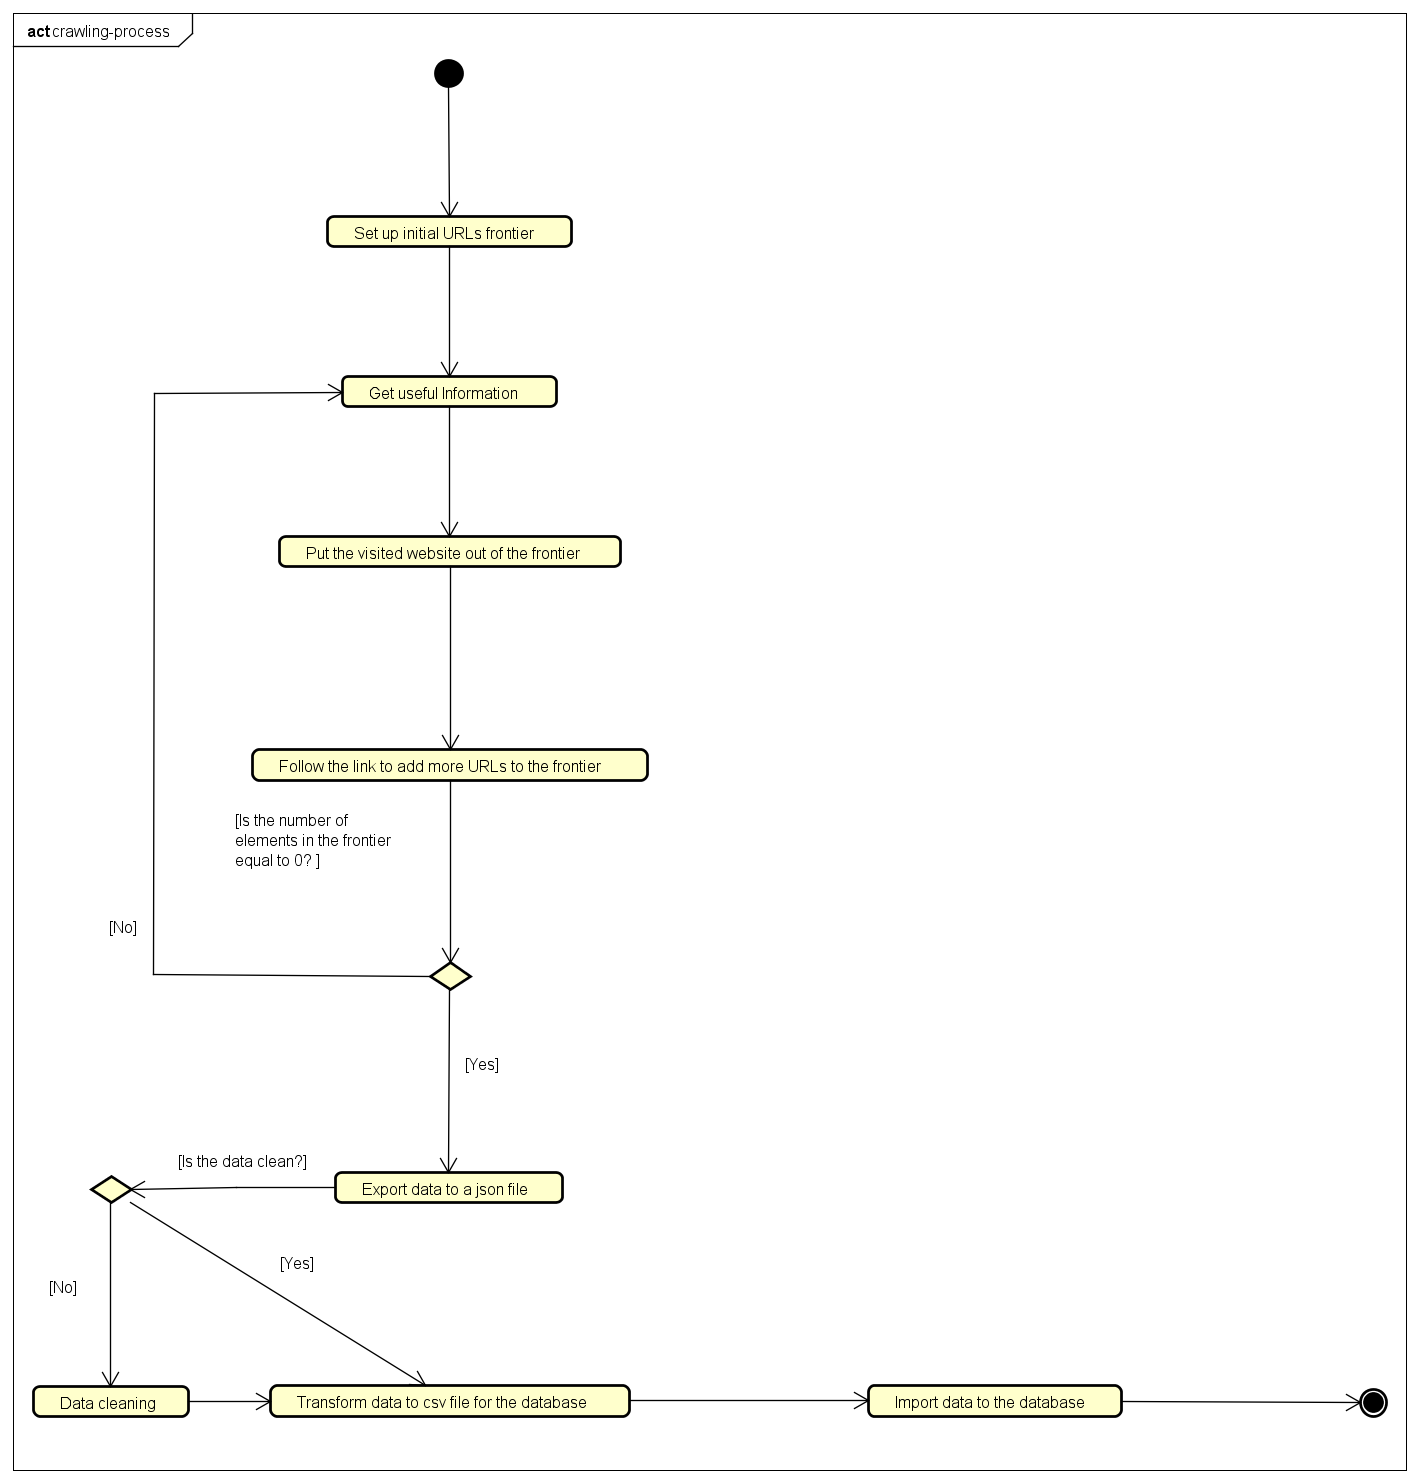
\includegraphics[width=\linewidth]{crawling-process.png}
    \caption{Detail figure about the crawling process}
  \end{subfigure}
  \begin{subfigure}[b]{0.4\linewidth}
    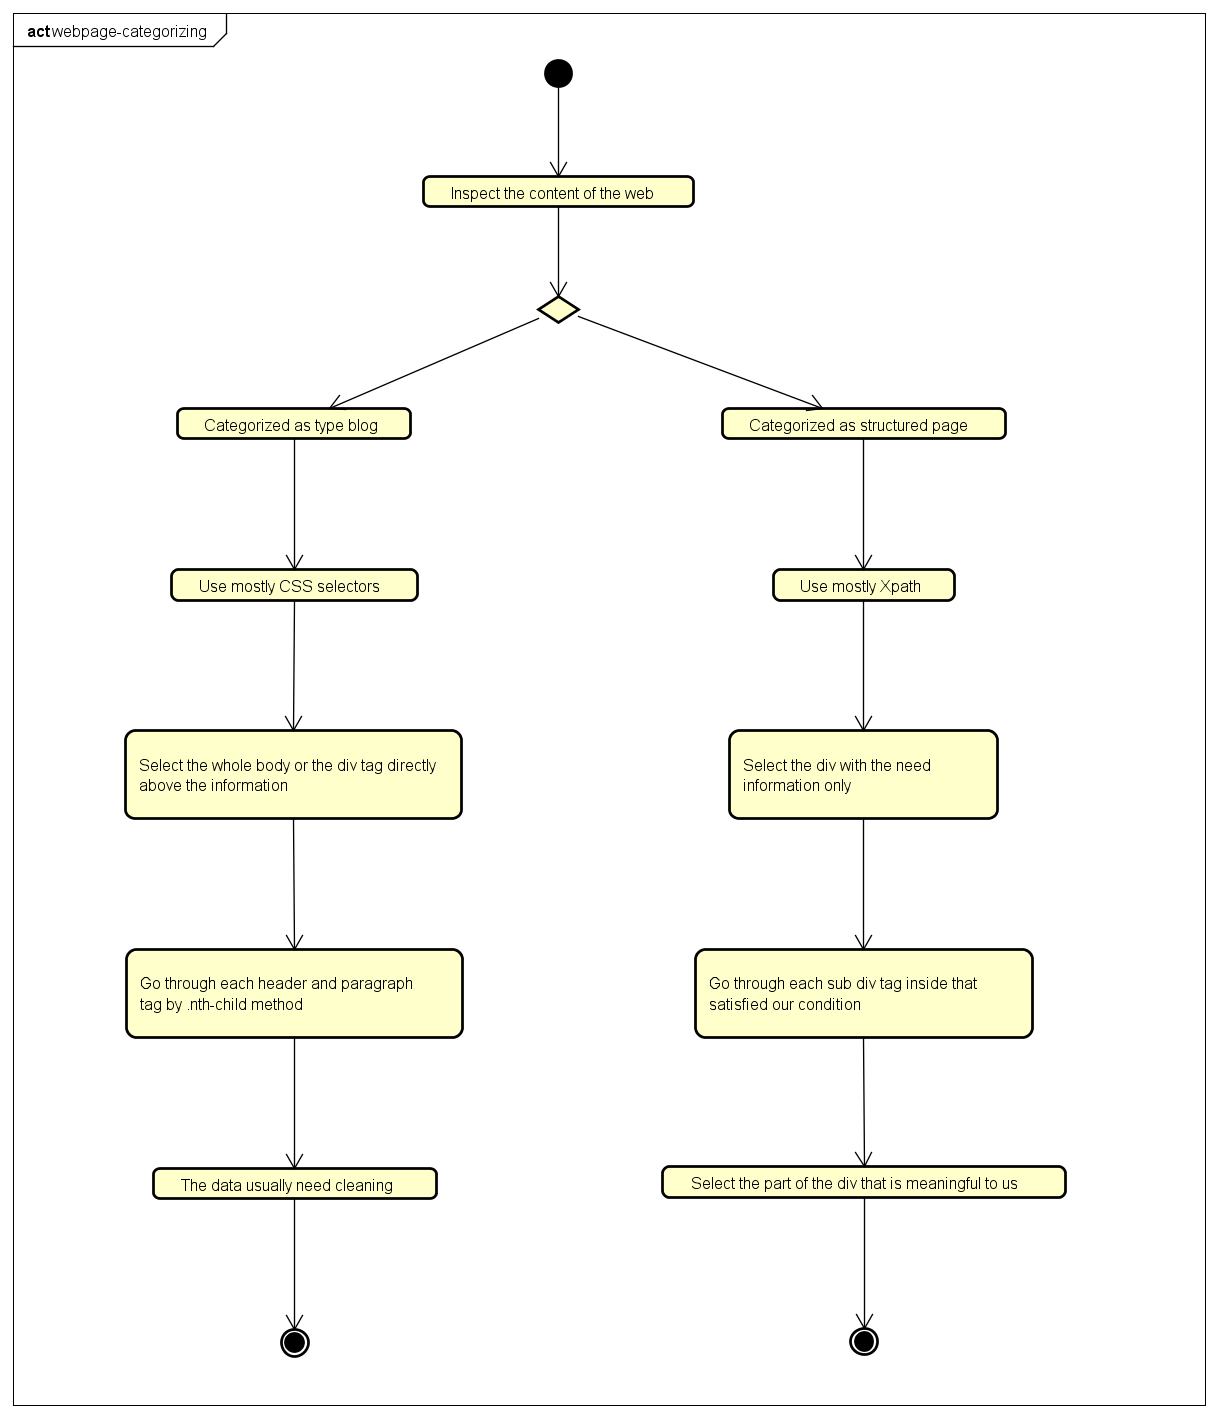
\includegraphics[width=\linewidth]{webpage-categorizing.png}
    \caption{The process of webpage categorizing}
  \end{subfigure}
  \caption{Crawling plan}
  \label{fig:cp}
\end{figure}
\subsection{Tools Used}
\begin{itemize}
	\item Crawler library; Scrapy (written in python)
	\item Additional libraries\footnote{all of which are python libraries}:
	\begin{itemize}
		\item json: to read and write json file
		\item BeautifulSoup: to pull data from html or xml document
		\item pandas: data manipulation tools
	\end{itemize}
	\item Database management system: postgresql\footnote{although it is not the fastest DBMS in the market but it works well with python} 
	\item Postgresql GUI tools: pgadmin
\end{itemize} 
\chapter{Web Crawler by Using Scrapy on Python}
\newpage
\section{Example problem: github page}
	\subsection{Goals}
	The goal of this problem is to familiarize with how scrapy works
	\subsection{Website classification}
	Github website is a structured website thus it better for our crawler to use the xpath selector. But to familiarize with how scrapy works, I choose to use the css selector.
	\subsection{Result}
	The end result is a json file containing title of the repository, Url to that repository, and last modified date of all the public repository in \href{https://github.com/vietanhdev?tab=repositories}{Github}. You can find out the result at \href{https://github.com/lam1910/crawler-gr1/blob/master/github-1303-vietanh.json}{json result}
\section{First website: travelling blog}
	\subsection{Goals}
	The goal of this problem is to get the user experiences when travelling in Vietnam via their travelling blog.
	\subsection{Website classification}
	This is a blog website with simple structure. It only contains a big div for css to make the website more beautiful. The information is stored on p tags with the titles is on the h3 and h4 tags.
	\subsection{Result}
	The end result is a csv file containing title of the experiences, places that he or she pass in Vietnam, and and the paragraph about the experiences. You can find out the result at \href{https://github.com/lam1910/crawler-gr1/blob/master/world-travel-family/world-travel-family.csv}{blog result}
\section{Second website: tripadvisor page}. There is a sql file to create a database using postgresql with the csv.
	\subsection{Goals}
	The goal of this problem is to get the user rating of each places they visited when travelling in Vietnam via a community rating system on tripadvisor.
	\subsection{Website classification}
	This is a well-defined structure website. This type of website usually built using a open-source framework like node.js. It has multiple div tags and inside those tags there are a lot of other tag. Each location is also on a div tag of their own. The information (the rating) is stored on the attribute on an a tag inside each individual div tags.
	\subsection{Result}
	The result is a detail database on places and rating of that places on 6 famous tourist cities in Vietnam Hanoi, Ho Chi Minh city, Danang, Hue, Hoian, and Sapa. This information is stored on the csv with each line containing the name of the city, the type of the places, the name of the place and its rating. You can find out the result at \href{https://github.com/lam1910/crawler-gr1/blob/master/trip-advisor/trip-data.csv}{tripadvisor data}. There is a sql file to create a database using postgresql with the csv.
\end{document}

